\documentclass{article}
\usepackage[russian]{babel}
\usepackage[utf8]{inputenc}
\usepackage{graphicx}
\usepackage{float}

\usepackage{geometry}
\geometry{a4paper, total={170mm,257mm}, left=30mm, right=25mm, top=30mm, bottom=10mm}

\setlength{\parskip}{0.6em}

\title{Анализ графа социальных связей в МФТИ}
\author{Андрей Сандлер}

\begin{document}

\maketitle

Недавно меня посетила одна мысль - у меня почти совсем нет друзей с ФФКЭ и ФПФЭ. Я так понимаю, что я не один такой с ФИВТа :) Развивая эту
мысль, я подумал, как можно было бы проверить, сколько друзей с разных факультетов есть у каждого физтеха? Ответ прямо под рукой --- ВКонтакте!

Итак, я решил поизучать граф дружеских связей на Физтехе, используя данные сайта vk.com. Тут уместно сделать некоторые пояснения.

Во-первых, подсчет друзей каждого человека даст много информации, а в итоге из-за её огромного количества не будет видно общей картины.
Поэтому лучше будет собрать некоторую статистику с ребер "графа дружбы". Например, почему бы не подсчитать, сколько ребер проведено между
факультетами? Это куда как глобальнее, и, в принципе, отражает среднее количество друзей с разных факультетов.

Но количества ребер мне мало, поскольку факультеты по численности бывают разные, и число ребер без учета количества человек ничего не
скажет. Как учесть размер факультета? Подумав, я решил считать плотность графа, то есть на ребре между ФИВТ и ФФКЭ писать плотность
двудольного графа, где вершины одной доли --- это фивты, а вершины другой доли --- кванты. Это число получалось маленьким, поэтому я его умножал
на 10000.

Возникает один технический вопрос: как по данным со страницы понять, является ли человек студентом Физтеха? Многие (но не все) указывают
МФТИ(ГУ) или МФТИ(ГУ) (см. в Москве) в качестве вуза на своей странице. Факультет чаще всего указывается вместе с вузом. Используя эти данные
и год выпуска, можно предположительно понять, учится ли человек в МФТИ.

И, наконец, как эти самые данные получить? ВКонтакте уже давно решили вопрос с парсингом страниц и придумали VK API. Оно умеет отдавать
список друзей человека, в котором есть поля <<вуз>>, <<факультет>>, <<год выпуска>>, и вообще всё, что можно указать на странице. Чтобы
воспользоваться этим API, нужно завести на своей страничке пустое приложение, а данные этого приложения отдать библиотеке, которая умеет
работать с VK API. Я нашел на Github библиотеку, написанную на моем любимом Ruby, и дело оставалось за малым --- запустить поиск в ширину и
ждать результатов.

Результаты заставили себя ждать 15 минут. Оказывается, мой BFS обошел две тысячи человек, найдя между ними чуть больше 60000 ребер. Неплохо!
Но мне показалось, что я получил не полную информацию о графе дружбы, поэтому я запустил поиск с трех других аккаунтов (ФИВТ, ФУПМ, ФАКИ), и
нашел ещё 10000 ребер. Как это получилось, я до сих пор не понимаю. Вроде бы все четверо (включая меня) состоят в друзьях друг у друга в
контакте, списки друзей принудительно открыты несколько месяцев назад, но все же поиск куда-то не доходит. Очень странное явление (возможно,
это следствие того, что часть друзей можно скрыть).

Тем не менее, результаты получены, таблицы заполнены, давайте на них смотреть.

\newpage

\begin{figure}[h]
\begin{center}
    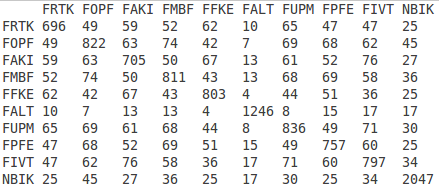
\includegraphics[height=5cm]{friendship_txt.png}
    \caption{Плотность графа дружеских связей между факультетами}
\end{center}
\end{figure}

Что сразу бросается в глаза? Числа на диагонали значительно больше, чем остальные, что и понятно --- друзей со своего факультета обычно
больше. Второе, что очень заметно --- это ФАЛТ. Внутренняя плотность там (и на НБИКе) огромная, а внешняя --- очень маленькая. География
сказывается.

\begin{figure}[h]
\begin{center}
    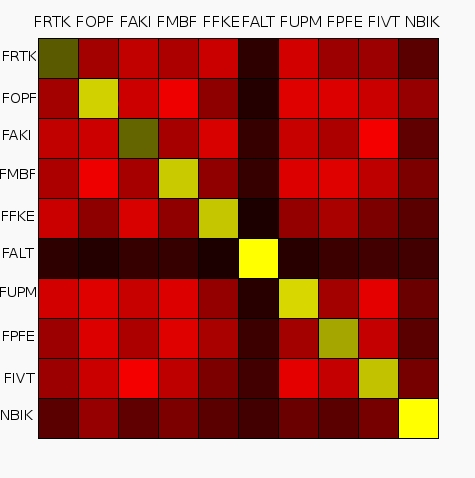
\includegraphics[height=10cm]{friendship_color.png}
    \caption{Плотность графа дружеских связей между факультетами, цветная версия}
\end{center}
\end{figure}

Глянем на цветную картинку. Желтым здесь обозначена внутренняя плотность, красным - внешняя, градация цвета от темного к
светлому означает величину плотности.

Получилось, что ФРТК и ФАКИ не очень дружны внутри. Интересно, как это на самом деле? ФОПФ дружит с ФМБФ, ФИВТ --- с ФАКИ (туда на ПМФ
переводятся) и с ФУПМом (исторически получилось). НБИК и ФОПФ довольно хорошо общаются.

\newpage

Так, а сколько же человек с каждого факультета сидит в контакте?

\begin{table}[ht]
\caption{Количество студентов МФТИ по факультетам}
\begin{center}
\begin{tabular}{|l|l|}
\hline
FUPM & 362 \\ \hline
FOPF & 308 \\ \hline
FAKI & 302 \\ \hline
FRTK & 296 \\ \hline
FIVT & 283 \\ \hline
FMBF & 247 \\ \hline
FPFE & 194 \\ \hline
FFKE & 177 \\ \hline
FALT & 110 \\ \hline
NBIK & 74  \\ \hline
     &     \\ \hline
TOTAL & 2353 \\ \hline
\end{tabular}
\end{center}
\end{table}

ФУПМ - очевидный лидер!

Что можно сказать по итогам исследования? Результаты показательные, но это отнюдь не значит, что на самом деле картина такая же - это всего
лишь статистика по данным ВКонтакте.

Надеюсь, было не очень скучно:)

Бонус для тех, кто дочитал: 10 самых "дружеобильных" людей с Физтеха (по данным vk.com):
\begin{itemize}
    \item Николай Синюхин, НБИК
    \item Леночка Обрайен, ФОПФ
    \item Георгий Речинский, ФУПМ
    \item Константин Виноградов, ФИВТ
    \item Егор Ефименко, ФОПФ
    \item Галка Болдырева, ФРТК
    \item Даша Милиженко, ФУПМ
    \item Михаил Ерохин, ФОПФ
    \item Андрей Криворучко, ФУПМ
    \item Анна Андреева, ФИВТ
\end{itemize}

\end{document}
